\documentclass[border=19pt,varwidth=30cm]{standalone}
\usepackage{graphicx,capt-of}
\usepackage{rotating}
\usepackage{multirow}
\usepackage[cm]{sfmath}

\renewcommand{\familydefault}{\sfdefault}

\newcounter{subfloat}
\renewcommand{\thesubfloat}{\Alph{subfloat}}
\newcommand{\image}[2]{%
    \stepcounter{subfloat}%
    \begin{tabular}[t]{@{}c@{}}
    \thesubfloat. #1 \\
    #2
    \end{tabular}%
}
\newcommand{\insertlabel}{%
    \Large
    \stepcounter{subfloat}%
    \thesubfloat}
\newcommand{\trm}[1]{\ensuremath{\textrm{\sffamily #1}}}

\begin{document}

\begin{figure}
    \centering
    \begin{tabular}{@{}lll@{}}
        \insertlabel & \insertlabel & \\
        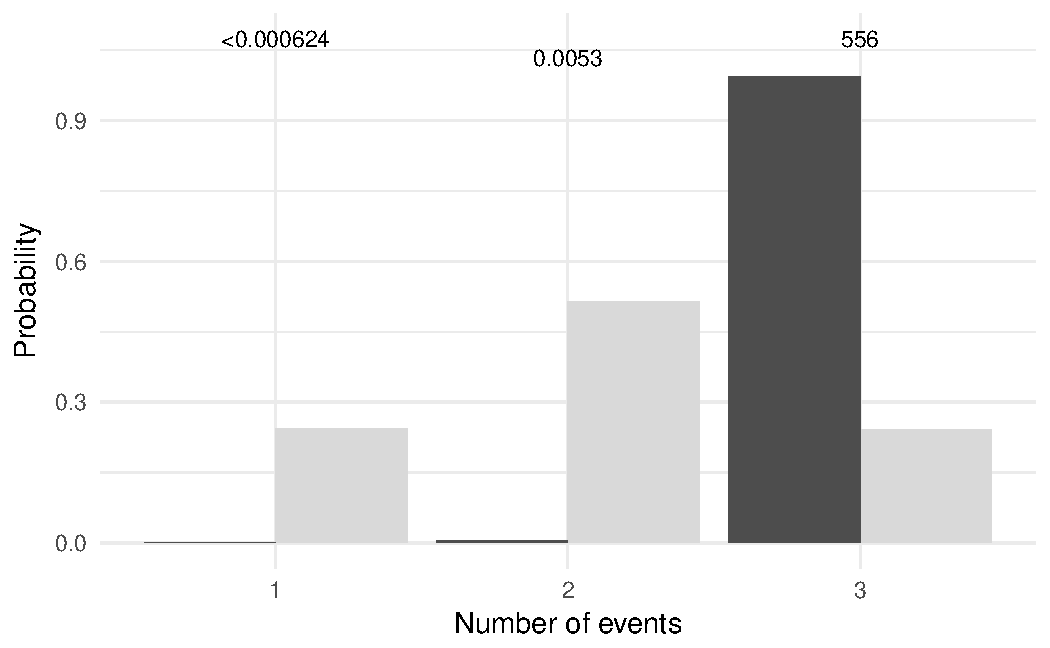
\includegraphics[width=0.46\textwidth]{./pycoevolity-nevents.pdf} &
        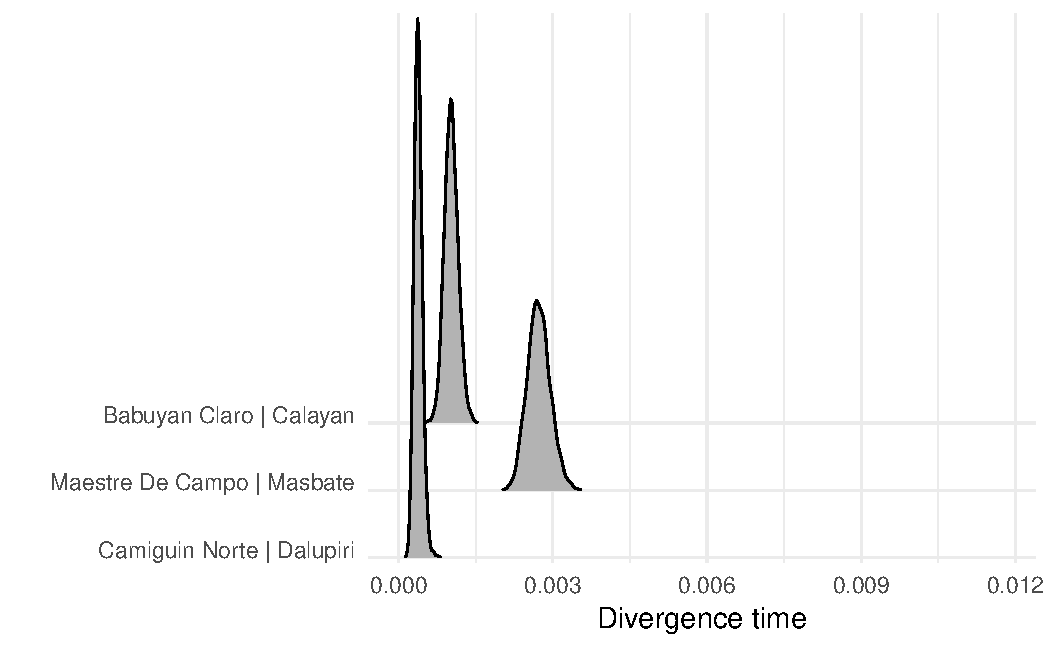
\includegraphics[width=0.46\textwidth]{./pycoevolity-times.pdf} &
        \multirow{1}{*}[19em]{\begin{rotate}{270}\Huge Ecoevolity\end{rotate}} \\
        \insertlabel & \insertlabel & \\
        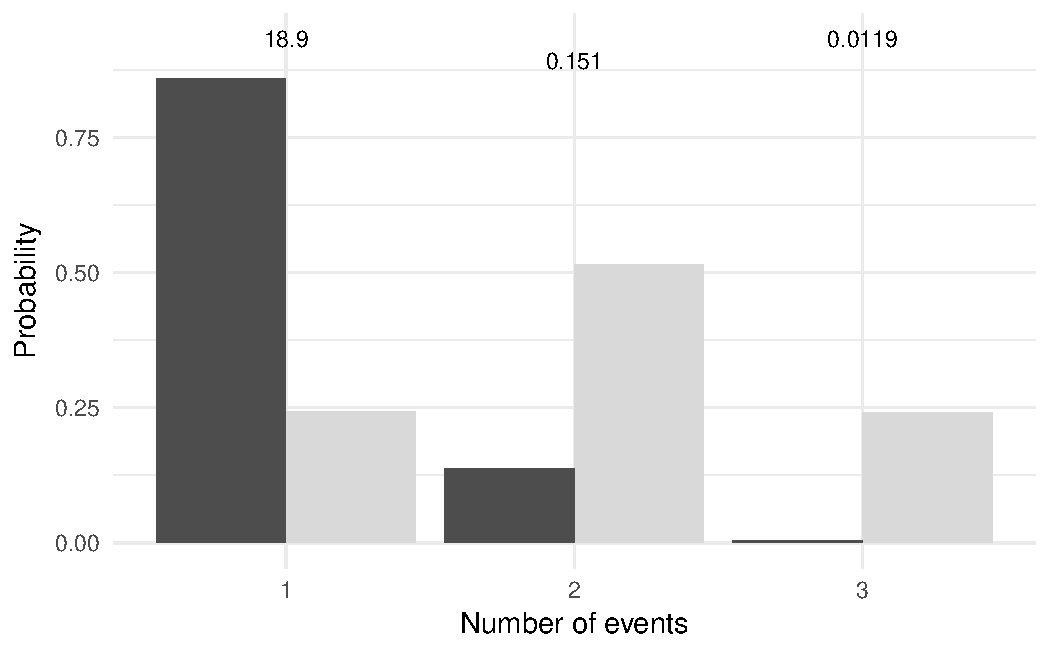
\includegraphics[width=0.46\textwidth]{./dppmsbayes-nevents.pdf} &
        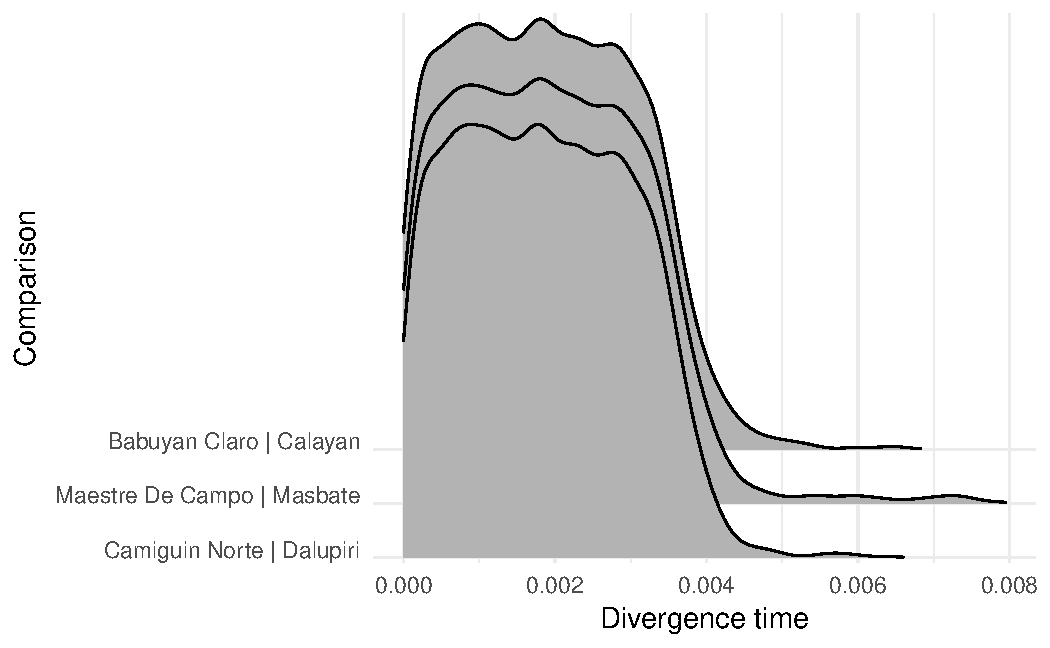
\includegraphics[width=0.46\textwidth]{./dppmsbayes-times.pdf} &
        \multirow{1}{*}[19em]{\begin{rotate}{270}\Huge dpp-msbayes\end{rotate}}
    \end{tabular}
\end{figure}

\end{document}
